\documentclass[11pt]{article}
\usepackage[margin=1in]{geometry}
\usepackage{amsmath,amssymb,amsthm}
\usepackage{booktabs}
\usepackage{graphicx}
\usepackage[hidelinks]{hyperref}
\newtheorem{proposition}{Proposition}
\newtheorem{corollary}[proposition]{Corollary}

\title{When Should an Agent Compact?\\Cache-Aware Rent-or-Buy Timing for LLM Agent Context}
\author{Anatole Seychal\\University of California, Berkeley\\\texttt{aseychal@berkeley.edu}}
\date{}

\begin{document}
\maketitle

\begin{abstract}
Long-running LLM agents periodically \emph{compact} their context, replacing history with a summary. The harnesses we examined trigger compaction at a fixed token count or a fixed fraction of the context window. We cast compaction \emph{timing} as a rent-or-buy problem under prompt-cache pricing. Held history pays cache-read rent on every call, while each compaction pays once for a summary and a cache rewrite. In steady state this is the Economic Order Quantity: the cost-optimal compaction point $H^\star$ depends on growth, summary cost and prices but not on the window. The cost curve is flat near $H^\star$, and window-relative triggers grow increasingly wasteful as windows grow.

We measure every term of the cost model on headless Claude Code (Sonnet 5.5). Measured this way, the model reproduces real bills to within 0.8\% on 18 pilot runs and on 12 held-out runs. At Claude Code prices and 3.6k tokens of growth per call, $H^\star\approx109$k of history, which makes Anthropic's 150k compaction default close to optimal. In trace-driven simulation of 1M-window sessions, compacting at 92\% of the window costs about 28\% more than compacting near $H^\star$.

We then ran 13 real sessions designed to cross $H^\star$, giving four paired task orderings. A fixed 150k trigger cost $9.8\%$ less than the default, and the online rule $2.8\%$ less; neither difference is statistically significant at $n=4$. Our recorded prediction of $-35\%$ failed. Its gap decomposes into an empirical bias correction we should not have applied (10 points) and back-loaded growth (16 points): real sessions do most of their growing just before they end.

In simulation, gating compactions on the predicted remaining session length is inert with learned predictors and worth at most 2 points even with an oracle. Steady-state savings are therefore a ceiling, not an expectation. The case for adaptive triggers is robustness across price regimes: a fixed 150k loses 29\% without caching.
\end{abstract}

\section{Introduction}
Agentic coding assistants run sessions of tens to hundreds of model calls, and their context grows with every tool result. Harnesses therefore \emph{compact}: they summarize or drop history so the session can continue. \emph{What} to keep has been studied extensively~\cite{complexitytrap,acon,tracer,compactiontheory}. \emph{When} to compact has received little formal treatment, though cache-aware systems touch on it~\cite{tokenpilot,cliff,infercept}.

In the products we examined the trigger is a constant~\cite{docs}:
\begin{itemize}
\item Claude Code compacts near the window limit by default. Its \texttt{--autocompact} option sets a compaction \emph{window} of at least 100k, and in our runs compaction fired about 70k below the value given.
\item Anthropic's compaction API defaults to 150k tokens.
\item OpenAI's Responses API exposes a \texttt{compact\_threshold}.
\item Gemini CLI's documented default is 70\% of the window.
\end{itemize}

The bill, however, is set by prices, growth and the cost of a compaction. Prompt caching makes held history cheap (0.05--0.1$\times$ the input price) but not free, and each compaction pays output price for the summary and rewrites part of the cached prefix at the write price.

\paragraph{Contributions.}
\begin{enumerate}
\item A cost model of compaction timing under prompt caching (\S\ref{sec:model}). Every term is measured from Claude Code usage logs, and the model reproduces real bills to within 1\%.
\item An EOQ characterization (\S\ref{sec:theory}):
  \begin{itemize}
  \item a closed-form, window-independent optimum, including re-fetch of dropped state;
  \item flatness, which bounds the cost of a mis-set trigger;
  \item the consequence that window-relative triggers grow increasingly wasteful as windows grow, while no single fixed threshold is robust across price regimes.
  \end{itemize}
  We also give a break-even (ski-rental) rule and an online steady-state rule that need no tuning, and a cold-cache rule.
\item Evaluation (\S\ref{sec:eval}):
  \begin{itemize}
  \item trace-driven simulation against product defaults, a hindsight-tuned threshold and an offline optimum;
  \item stress tests;
  \item two real-agent studies, including a prediction recorded before the runs that failed. A decomposition attributes the failure to growth that arrives late in the session.
  \end{itemize}
\item A negative result on horizon awareness (\S\ref{sec:horizon}): predicting the remaining session length adds at most 2 points.
\end{enumerate}

\section{Related work}
\paragraph{What to keep.} Observation masking matches LLM summarization on SWE-agent at about half the cost~\cite{complexitytrap}. ACON optimizes compression guidelines~\cite{acon}, TRACER learns per-tool retention~\cite{tracer}, and ARC replaces tool outputs with recoverable citations~\cite{arc}. Context-Folding learns to branch and fold~\cite{folding}, and MemGPT pages memory under model control~\cite{memgpt}. Tirmazi et al.\ relate compaction to one-way communication complexity~\cite{compactiontheory}; their analysis concerns the content of a bounded state, not timing or price. Liu finds that compression increases re-fetching~\cite{compresscost}, which is our $\rho$. We measure it at 0.7\% of dropped tokens for Claude Code on our tasks.

\paragraph{Cache-aware context management.} TokenPilot trades context sparsity against prefix-cache stability with lifecycle-based eviction~\cite{tokenpilot}, and CliffCompaction truncates rather than rewrites history~\cite{cliff}. Neither derives when a compaction pays for itself.

\paragraph{Online algorithms.} Our break-even rule is ski rental~\cite{karlin88,karlin94}. The horizon gate of \S\ref{sec:horizon} is in the spirit of learning-augmented ski rental~\cite{purohit18}, and the Bahncard problem~\cite{fleischer} is a close relative. InferCept decides whether to preserve, discard or swap KV cache during tool calls~\cite{infercept}. Our steady-state analysis is the Economic Order Quantity of inventory theory~\cite{harris}.

\section{Cost model}\label{sec:model}
All costs are in units of the base input-token price.

\paragraph{Prices.} Cache reads cost $r$ and cache writes $w$ ($1.25$ for 5-minute entries, $2$ for 1-hour entries). Outputs cost $o\approx5$.

\paragraph{Session.} A session has a static prefix $S$ and history $H$, which grows by $g$ tokens per call on average. Holding one history token for one call costs $h=r+q$, where $q$ is an optional context-rot price.

\paragraph{Compaction.} Compacting at $H$ leaves $s(H)=\sigma+\rho H$: a post-compaction conversation $\sigma$ plus re-fetched state $\rho H$. Only part of $\sigma$ is generated by the summary call; we write $\sigma_o\le\sigma$ for that part, and the rest is restored files and preserved messages. A compaction also evicts a part $S_r$ of the cached static prefix. The one-time buy cost is
\begin{equation}
K(H)=r(S+H)+o\,\sigma_o+(w-r)\,\bigl(s(H)+S_r\bigr)+P,
\end{equation}
where $P$ is an optional quality penalty.

\paragraph{Measured parameters.} We measured every term from Claude Code's usage counters: the per-call cache reads and writes, and the cumulative \texttt{modelUsage} totals.
\begin{itemize}
\item \textbf{Post-compaction conversation:} $\sigma\approx11$k (9--15k across compactions).
\item \textbf{Summary output:} the summary call generates $\sigma_o\approx5.2$k output tokens over 54 compactions. It rises with history size, from 4.4k at about 50k of context to 6.3k at 100--200k. The summary call reads the context from cache.
\item \textbf{Evicted prefix:} after a compaction only the cross-session part of the prefix (27.4k tokens of shared system prompt and tools) remains cached. The session-specific rest, $S_r\approx8.6$k of a 36k prefix, is rewritten.
\item \textbf{Re-fetch:} $\rho\approx0.007$. This is tool output re-read after a compaction for files already seen before it, divided by the history tokens dropped. It holds both for the pilot's small compactions and for the high-growth runs' 100--200k compactions.
\item \textbf{Cache prices:} Claude Code writes 1-hour cache entries ($w=2$), and Sonnet 5.5 reads cache at $r=0.05$.
\end{itemize}
Per-message usage in the CLI's stream under-reports output by roughly 5$\times$, so all dollar figures use \texttt{modelUsage}. Unless stated otherwise we use $S=40$k, $\sigma=11$k, $\sigma_o=5.2$k, $S_r=8.6$k and $\rho=0$.

\section{Theory}\label{sec:theory}

\begin{proposition}[Optimal compaction point]\label{prop:eoq}
Suppose $\sigma$ is constant, $S+H<W$ throughout, and a session compacts at $H$ and regrows over $n$ calls. Then $H=(\sigma+gn)/(1-\rho)$, and the trigger-dependent cost per call is
\[
f(n)=\frac{hgn(1+\rho)}{2(1-\rho)}+\frac{A'}{n},\qquad A'=rS+o\sigma_o+P+(w-r)S_r+\frac{w\sigma}{1-\rho}.
\]
Minimizing gives
\[
n^\star=\sqrt{\frac{2A'(1-\rho)}{hg(1+\rho)}},\qquad H^\star=\frac{\sigma+gn^\star}{1-\rho}.
\]
For $\rho=0$ this is $H^\star=\sigma+\sqrt{2gA/h}$ with $A=rS+o\sigma_o+w\sigma+(w-r)S_r+P$. As long as $S+H^\star<W$, $H^\star$ does not depend on the window.
\end{proposition}

At Claude Code prices, $H^\star\approx54$k at $g=700$ tokens per call (our pilot) and $\approx109$k at $g=3.6$k (our sessions). The closed form agrees with a numerical minimization of the exact steady-state cost to within 2\% across price regimes, $\rho\in\{0,0.1,0.3\}$, and $g$ from 500 to 8k (unit-tested). Figure~\ref{fig:hstar} shows $H^\star$ against growth for four price regimes.

\begin{proposition}[Flatness]\label{prop:flat}
$f(xn^\star)/f(n^\star)=(x+1/x)/2$.
\end{proposition}
A trigger within $2\times$ of $n^\star$ therefore pays at most 25\% more of the \emph{trigger-dependent} cost; the share of the total bill is smaller (Figure~\ref{fig:flat}).

\begin{corollary}[Window-relative triggers]\label{cor:window}
A trigger at fraction $\tau$ of the window has $x\approx(\tau W-S-\sigma)/(H^\star-\sigma)$, so its steady-state excess grows linearly in $W$. At Claude Code prices with $g=3.6$k, compacting at 967k gives $x\approx9.4$, or $4.7\times$ the optimal trigger-dependent cost; at $g=700$, $x\approx21$ ($10.6\times$). The 150k API default gives $x\approx1.0$ at $g=3.6$k, but $x\approx2.3$ ($1.37\times$) at $g=700$. Finite sessions cap the realized excess, because a session that ends before the trigger fires never pays it (\S\ref{sec:real}).
\end{corollary}

\begin{proposition}[No robust fixed threshold]\label{prop:robust}
For a fixed threshold $H_0$, $x=(H_0-\sigma)/(H^\star-\sigma)$, and $H^\star-\sigma=\sqrt{2gA/h}$ at $\rho=0$. Hold $\sigma$ fixed, and suppose $gA/h$ spans a factor $F$ across the regimes a product serves. Then every fixed threshold has $\max(x,1/x)\ge F^{1/4}$ in some regime, and its excess there is at least $(F^{1/4}+F^{-1/4})/2$.
\end{proposition}

\begin{proposition}[Break-even tracks the optimum]\label{prop:be}
Let $\sigma$ be constant and $\rho=0$. The ski-rental rule compacts once the accumulated rent on the compactable excess, $h\sum_k (H_k-s(H_k))$, reaches $K(H)$. It fires at
\[
n_{BE}=(b/h-\tfrac12)+\sqrt{(b/h-\tfrac12)^2+(n^\star)^2}\;\le\;n^\star+2b/h,\qquad b=r\le h,
\]
that is, within two calls of $n^\star$ (one call when $q=0$), without knowing $g$.
\end{proposition}
For $\rho>0$ we report break-even's behavior empirically. We do not claim worst-case competitive ratios for the multi-cycle problem, because the buy cost rises over time and rent continues after each buy.

\begin{proposition}[Cold-cache rule]\label{prop:cold}
After an idle gap longer than the cache TTL, not compacting rewrites $S+H$ at price $w$. Compacting instead reads $S+H$ once uncached for the summary, pays $o\sigma_o$, and writes $S+s$. Compaction is therefore immediately profitable when
\[
(w-1)(S+H)>o\sigma_o+w(S+s)+P.
\]
With our measured parameters this means $H>88$k for 1-hour entries and $H>319$k for 5-minute entries.
\end{proposition}

\begin{figure}[t]
\centering
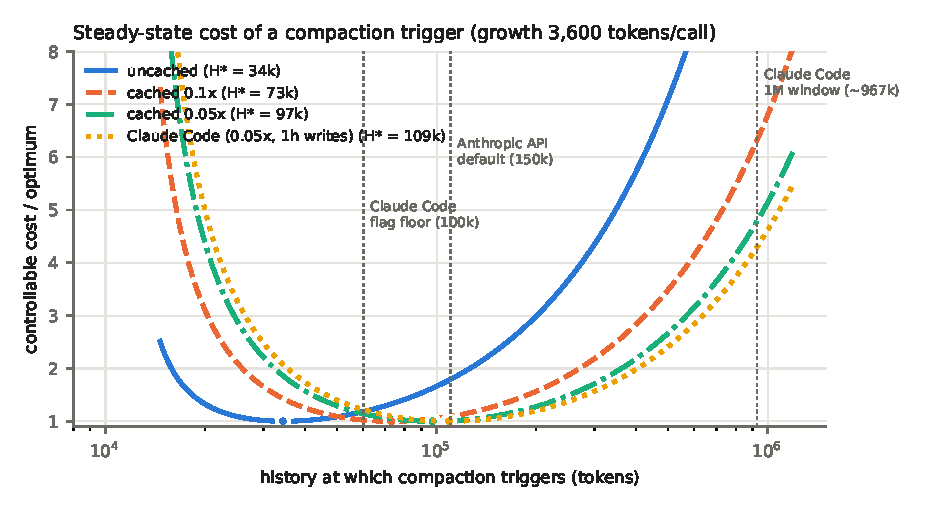
\includegraphics[width=\linewidth]{figures/flatness.pdf}
\caption{Steady-state cost of a fixed compaction trigger relative to the optimum at 3.6k tokens of growth per call, with $S=40$k and the measured compaction costs. Window-relative product triggers sit far to the right of every minimum.}
\label{fig:flat}
\end{figure}

\begin{figure}[t]
\centering
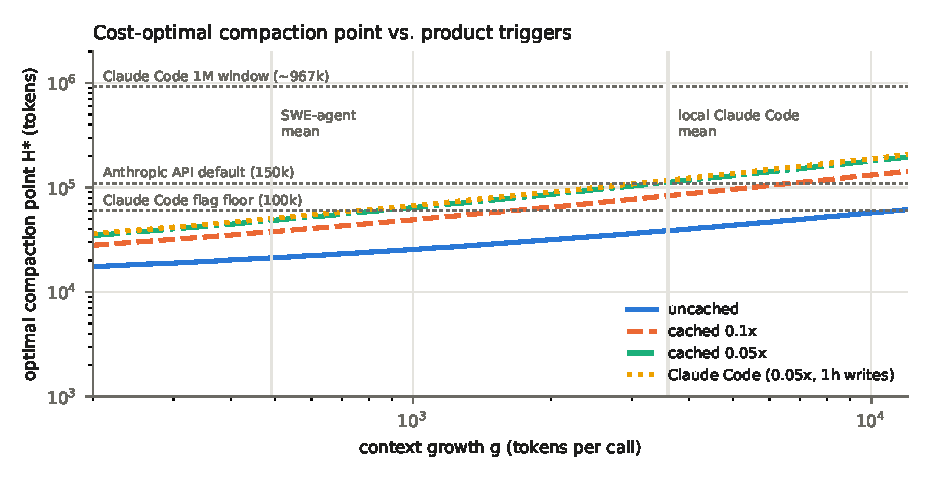
\includegraphics[width=\linewidth]{figures/optimum_vs_growth.pdf}
\caption{Cost-optimal compaction point $H^\star$ versus growth per call, for four price regimes. Dashed lines are product triggers expressed as history.}
\label{fig:hstar}
\end{figure}

\section{Evaluation}\label{sec:eval}

\paragraph{Data.}
\begin{itemize}
\item \textbf{Claude Code sessions.} 25 of our own sessions, reduced to numeric token usage only: 1{,}490 calls, mean growth 3.6k tokens per call, a median of 36 calls, and 94.7\% of input tokens served from cache. These come from one user. Twelve are subagent sessions, and the calls span four models (Fable 5.1, Opus 5.5, Sonnet 5.5, Fable 5); we apply Claude Code prices to all of them.
\item \textbf{SWE-agent trajectories.} 1{,}500 trajectories sampled from 13{,}287 in two public shards~\cite{nebius}, with mean growth 491 tokens per call. Token counts are approximated as characters divided by 4. Summaries are assumed to be 2k tokens, all of them generated, since these contexts peak near 10k.
\end{itemize}

\paragraph{Policies.}
\begin{itemize}
\item Fixed 92\% of the window, the reference for reported changes.
\item The product defaults: 150k of total context and 70\% of the window.
\item Deterministic break-even.
\item The online rule: Proposition~\ref{prop:eoq} solved numerically with a running mean of $g$, with no tuning to the data.
\item The best fixed threshold, chosen in hindsight from an independent 48-point grid on the evaluation data.
\item An offline optimum, computed by beam DP over compaction times.
\end{itemize}
``Claude Code'' price rows use $w=2$ and the measured compaction costs, and do not simulate cache expiry except in the cold-cache experiment. Synthetic sessions resample per-call growth i.i.d.\ from the local traces, so they do not reproduce growth that arrives late in a session; \S\ref{sec:real} shows why that matters.

\begin{table}[t]
\centering
\small
\caption{Cost change (\%) vs.\ a fixed 92\%-of-window trigger; negative is cheaper. $H^\star$ is the online rule's target at the dataset's mean growth. ``Best fixed'' is tuned in hindsight on the evaluation data. Synthetic rows use 300 sessions resampled from the local traces, or 1{,}500 SWE-agent trajectories.}
\label{tab:main}
\resizebox{\linewidth}{!}{\begin{tabular}{lllrrrrrrr}
\toprule
Data & Prices & $W$ & $H^\star$ & 150k ctx & 70\%$W$ & Break-even & Online & Best fixed & Opt.\\
\midrule
Claude Code & uncached & 200k & 35k & $-9.7$ & $-12.6$ & $-29.3$ & $-29.7$ & $-30.0$ (31k) & $-31.5$\\
Claude Code & cached 0.1$\times$ & 200k & 73k & $-3.7$ & $-4.7$ & $-6.0$ & $-6.0$ & $-6.2$ (67k) & $-8.4$\\
Claude Code & cached 0.05$\times$ & 200k & 98k & $-1.5$ & $-1.7$ & $-1.4$ & $-1.2$ & $-1.5$ (106k) & $-3.6$\\
Claude Code & Claude Code & 200k & 109k & $-0.8$ & $-0.8$ & $-0.7$ & $-0.8$ & $-0.8$ (124k) & $-2.7$\\
Claude Code & uncached & 1M & 35k & $-56.7$ & $-6.3$ & $-65.9$ & $-66.3$ & $-66.4$ (31k) & $-67.1$\\
Claude Code & cached 0.1$\times$ & 1M & 73k & $-37.4$ & $-4.4$ & $-38.6$ & $-38.8$ & $-38.9$ (67k) & $-40.4$\\
Claude Code & cached 0.05$\times$ & 1M & 98k & $-25.9$ & $-3.3$ & $-25.6$ & $-25.7$ & $-25.9$ (106k) & $-27.5$\\
Claude Code & Claude Code & 1M & 109k & $-21.7$ & $-2.9$ & $-21.4$ & $-21.6$ & $-21.8$ (124k) & $-23.2$\\
SWE-agent & uncached & 32k & 6k & $+0.4$ & $-12.7$ & $-41.0$ & $-41.0$ & $-40.3$ (6k) & $-43.2$\\
SWE-agent & cached 0.1$\times$ & 32k & 17k & $-0.4$ & $+2.9$ & $-1.5$ & $-0.9$ & $-0.5$ (16k) & $-6.0$\\
SWE-agent & cached 0.05$\times$ & 32k & 23k & $-0.7$ & $+8.5$ & $+0.8$ & $+0.3$ & $-0.7$ (31k) & $-2.6$\\
SWE-agent & Claude Code & 32k & 27k & $-0.8$ & $+10.6$ & $+0.0$ & $-0.4$ & $-0.8$ (31k) & $-2.0$\\
SWE-agent & uncached & 128k & 6k & $+0.0$ & $+0.0$ & $-41.4$ & $-41.4$ & $-40.7$ (6k) & $-43.5$\\
SWE-agent & cached 0.1$\times$ & 128k & 17k & $+0.0$ & $+0.0$ & $-0.7$ & $-0.0$ & $+0.0$ (36k) & $-5.2$\\
SWE-agent & cached 0.05$\times$ & 128k & 23k & $+0.0$ & $+0.0$ & $+2.0$ & $+1.6$ & $+0.0$ (36k) & $-1.4$\\
SWE-agent & Claude Code & 128k & 27k & $+0.0$ & $+0.0$ & $+1.3$ & $+0.8$ & $+0.0$ (36k) & $-0.8$\\
Replay (25) & Claude Code & 1M & 110k & $-22.1$ & $-1.1$ & $-22.5$ & $-22.6$ & $-22.8$ (145k) & $-24.4$\\
\bottomrule
\end{tabular}
}
\end{table}

\paragraph{Simulation results} (Table~\ref{tab:main}).
\begin{itemize}
\item \textbf{Online rule vs.\ hindsight.} With i.i.d.\ growth, the online rule is within 1.6\% of the hindsight-tuned threshold in all 17 settings.
\item \textbf{1M windows.} At a 1M window with Claude Code prices, the 92\% trigger costs about 28\% more than the online rule: the rule is 21.6\% cheaper on synthetic sessions and 22.6\% cheaper replaying our 25 sessions. With 0.1$\times$ caching the rule is 38.8\% cheaper, and without caching 66\%.
\item \textbf{200k windows.} With Claude Code prices every trigger is within 1\% of the best, because 92\% of 200k is already close to $H^\star$. The 150k default matches the online rule at our sessions' growth.
\item \textbf{SWE-agent.} For slow-growing SWE-agent sessions, the 70\%-of-window trigger costs up to 10.6\% more at 32k, while the online rule stays within 1.6\% of the best.
\item \textbf{Transfer.} A threshold tuned once (83k, optimal for 0.1$\times$ caching) costs 8.6--9.2\% more when a quality penalty is added and 16.5\% more without caching. The online rule stays within 0.5\% of the per-regime best.
\item \textbf{Summary size.} As summaries vary from 2k to 20k at $\rho=0$, the online rule beats the 150k default by at most 1.5\%. Only with substantial re-fetch ($\rho=0.3$, far above the measured 0.007) does the gap reach 3.8\%.
\item \textbf{Cold-cache rule.} Assuming idle gaps exceed an hour before 1.5\% of calls (a rate taken from our session logs, which the released traces do not contain), adding Proposition~\ref{prop:cold} to the 92\% trigger at 1M cuts its cost by 17\%. The online rule gains 0.3\%, because it keeps contexts small.
\end{itemize}

\paragraph{Stress tests} (Table~\ref{tab:worst}). We draw 150 sessions from three families (constant, heavy-tailed, and a low-to-high growth switch) and evaluate every prefix, so a session may end right after a compaction. These are random hard cases, not adversaries constructed against each policy. The online rule and break-even stay within $1.15\times$ of the offline optimum. The 92\% trigger reaches $1.52\times$ at 1M, a fixed 30k threshold $1.66\times$, and randomized break-even $2.05\times$ at 200k.

\begin{table}[t]
\centering
\small
\caption{Stress-test ratios (cost / offline optimum) over every prefix of 150 sessions drawn from steady, heavy-tailed and switching growth families.}
\label{tab:worst}
\begin{tabular}{lrrrr}
\toprule
Policy (Claude Code prices) & max, 200k & max, 1M & p99, 1M & mean, 1M\\
\midrule
online steady-state & 1.140 & 1.140 & 1.123 & 1.020\\
break-even & 1.146 & 1.146 & 1.115 & 1.013\\
online, recent $g$ (exploratory) & 1.155 & 1.155 & 1.117 & 1.014\\
online, recent $g$ + horizon gate & 1.155 & 1.155 & 1.117 & 1.014\\
fixed 80k history & 1.220 & 1.220 & 1.143 & 1.031\\
randomized break-even & 2.054 & 1.430 & 1.203 & 1.033\\
fixed 92\% of window & 1.181 & 1.520 & 1.456 & 1.068\\
fixed 30k history & 1.658 & 1.658 & 1.569 & 1.236\\
\bottomrule
\end{tabular}

\end{table}

\paragraph{Real-agent pilot.} We drive Claude Code (Sonnet 5.5) headlessly through 13- or 25-message sessions.
\begin{itemize}
\item \textbf{Task.} Twelve standard-library modules each carry one injected bug, reported vaguely one message at a time. The long variant adds twelve test-writing requests.
\item \textbf{Probes.} Rules stated only in the first message test whether compaction drops instructions. A final request asks for each fix's original buggy expression, which cannot be recovered once the bug is fixed.
\item \textbf{Scoring.} Hidden differential tests compare each module against the untouched original.
\item \textbf{Controller.} An external controller sends \texttt{/compact} between turns whenever its policy fires.
\end{itemize}
Table~\ref{tab:pilot} reports the results. The economic arm's target, about 54k of history, was never reached, so it behaved like \emph{auto}. Compacting at 15k of history (about $1.4\sigma$, so each compaction removed only 2--5k tokens of context) raised cost by 32\% and 143\%, as flatness predicts for $x\ll1$. Recall was 9.7 vs.\ 11.7 of 12 after about nine compactions, which is descriptive at $n=3$. Replaying each run's observed growth and compaction points with the measured parameters reproduces its cost to within 0.8\% mean absolute error. Uncompacted runs are within 0.1\%, and compacted runs within 5\%.

\begin{table}[t]
\centering
\small
\caption{Real-agent pilot, Claude Code (Sonnet 5.5), three task orderings per row, means with min--max cost. Every run fixed all 12 bugs, and none created files in \texttt{pkg/}.}
\label{tab:pilot}
\begin{tabular}{llrrrrr}
\toprule
Session & Arm & Cost (\$) & vs.\ auto & Compactions & Recall /12 & Untagged\\
\midrule
13 msgs & auto (window) & 0.55 (0.52--0.57) & --- & 0.0 & 12.0 & 0.0\\
13 msgs & economic & 0.56 (0.52--0.59) & $+1.7\%$ & 0.0 & 11.3 & 0.0\\
13 msgs & at 15k history & 0.73 (0.71--0.74) & $+32.3\%$ & 2.0 & 12.0 & 0.0\\
25 msgs & auto (window) & 0.97 (0.83--1.13) & --- & 0.0 & 11.7 & 0.0\\
25 msgs & economic & 0.98 (0.95--1.03) & $+1.4\%$ & 0.0 & 12.0 & 0.0\\
25 msgs & at 15k history & 2.36 (1.83--2.97) & $+142.7\%$ & 9.3 & 9.7 & 0.3\\
\bottomrule
\end{tabular}
\end{table}

\subsection{Real sessions past \texorpdfstring{$H^\star$}{H*}}\label{sec:real}
\paragraph{Workload.} We extended the task so that sessions cross $H^\star$:
\begin{itemize}
\item eight further bugs in large standard-library modules (1.4--3.3k lines), reported by symptom only;
\item eight end-to-end audit requests, each requiring the module's exact line count and last top-level definition, which certifies a full read;
\item a rule introduced at message 10.
\end{itemize}
Uncompacted (\emph{auto}) sessions ran about 110 calls at about 3.0k tokens of growth per call, peaking near 365k. A truncated calibration run had shown 5.4k per call.

\paragraph{Arms.} We compare three arms:
\begin{itemize}
\item \emph{auto}, the CLI default on a 1M window, which never fired;
\item the online rule, which chose its compaction points with the cost model as it stood before the corrections of \S\ref{sec:model};
\item an external trigger at 150k of total context.
\end{itemize}
Claude Code's own \texttt{--autocompact 150000} fired at 69--85k, so we did not use it.

\paragraph{Protocol and attrition.} Before the runs we committed predictions to the repository (commit \texttt{cd8e116}). That is a dated record, not an external registry. Table~\ref{tab:prereg} lists every prediction and its outcome. We deviated from the recorded plan in three ways:
\begin{itemize}
\item 20 bugs instead of 24;
\item an external 150k trigger instead of the CLI's;
\item four paired orderings instead of five.
\end{itemize}
The fifth ordering (h4) completed only under the 150k arm. Its other runs stalled in three attempts, on which the logs show the account's five-hour rate-limit window saturated. Fourteen throttled partial runs (\$18.06) are excluded but archived. We report only the four complete orderings. At $n=4$ the exact two-sided permutation test cannot go below $p=0.125$.

\begin{table}[t]
\centering
\small
\caption{Predictions recorded before the high-growth runs, and outcomes (four paired orderings; paired-$t$ 95\% CIs).}
\label{tab:prereg}
\begin{tabular}{p{0.42\linewidth}p{0.48\linewidth}}
\toprule
Recorded prediction & Outcome\\
\midrule
Online rule vs.\ \emph{auto}: $-35\%\pm6\%$ & $-2.8\%$ ($-21.9$ to $+16.3$): failed\\
Online rule vs.\ 150k: within $\pm5\%$ & $+8.1\%$ ($-8.6$ to $+24.7$): point estimate outside\\
Far arm (3$\times H^\star$) vs.\ \emph{auto}: $-22\%\pm8\%$ & not run\\
Bugs fixed: no worse than 23/24 & 20/20 in every run (20-bug variant): met\\
Recall drop: at most 1/12 & 150k: $-1.5$/20; online: $-4$/20: failed\\
\bottomrule
\end{tabular}
\end{table}

\paragraph{Results} (Table~\ref{tab:hg}). Against \emph{auto}:
\begin{itemize}
\item the 150k trigger cost $9.8\%$ less (paired-$t$ 95\% CI $-25.8$ to $+6.3$; exact permutation $p=0.25$);
\item the online rule cost $2.8\%$ less ($-21.9$ to $+16.3$; $p=0.75$);
\item the online rule cost $8.1\%$ more than the 150k trigger.
\end{itemize}
Every run fixed all 20 bugs and violated no rule. Recall of the exact buggy expressions was 19.0, 17.5 and 15.0 of 20 for the three arms, which is descriptive given $n=4$ and the confound between arm and compaction count. The cost model, with parameters measured on the pilot alone, reproduces the 12 paired bills to within 0.8\%.

\begin{table}[t]
\centering
\small
\caption{Real sessions past $H^\star$: Claude Code (Sonnet 5.5), four paired orderings, means. Bill components in \$ per run from \texttt{modelUsage}. ``History'' is cache-read spend net of reading the static prefix. Recall counts exact buggy expressions reproduced at the end.}
\label{tab:hg}
\begin{tabular}{lrrrrrrr}
\toprule
Arm & Cost (\$) & vs.\ auto & Reads (history) & Writes & Output & Compactions & Recall /20\\
\midrule
auto & 3.25 & --- & 1.34 (0.95) & 1.36 & 0.54 & 0.0 & 19.0\\
150k & 2.91 & $-9.8\%$ & 0.84 (0.44) & 1.47 & 0.60 & 2.0 & 17.5\\
eoq & 3.13 & $-2.8\%$ & 0.82 (0.41) & 1.59 & 0.72 & 3.0 & 15.0\\
\bottomrule
\end{tabular}

\end{table}

\paragraph{Why the prediction failed.} Table~\ref{tab:gap} changes one assumption at a time.
\begin{itemize}
\item \textbf{Bias correction (10.3 points).} The recorded $-35\%$ applied the pilot's empirical bias correction. That correction compensated for two measurement artifacts, under-reported output and an overcharged summary, and should not have been applied.
\item \textbf{Cost-model correction (small).} Correcting the model itself moves the prediction by 1.5 points.
\item \textbf{Real growth and length (5.7 points).} The real sessions grew more slowly than planned.
\item \textbf{Back-loading (15.8 points, the largest effect).} In every session 87--89\% of growth arrived in the last 40\% of calls, so little of the session remains after $H^\star$ for any compaction to repay itself.
\end{itemize}
Replaying \emph{auto}'s real growth under the live online rule gives $-4.6\%$, close to the observed $-2.8\%$. Per ordering the agreement is loose (predicted $-8.6/-0.7/-5.0/-4.1$ vs.\ observed $-7.0/+14.7/-6.0/-12.8$), so the model is consistent with the outcome rather than predictive of individual runs. The bill breakdown shows the mechanism directly. Compaction cut history rent by more than half: it was 29\% of the \emph{auto} bill. The added cache writes and summary output won back 79\% of the online rule's read saving, but only 34\% of the 150k trigger's, which compacted less often.

\begin{table}[t]
\centering
\small
\caption{Online rule vs.\ \emph{auto}, changing one assumption at a time (\texttt{experiments/prediction\_gap.py}).}
\label{tab:gap}
\begin{tabular}{lr}
\toprule
Setting & Change\\
\midrule
As recorded: pre-correction model, i.i.d.\ synthetic growth, 4k/call, 120 calls, bias-corrected & $-34.9\%$\\
Without the bias correction & $-24.6\%$\\
Corrected cost model & $-26.1\%$\\
Real growth and session length, call order shuffled & $-20.4\%$\\
Real growth in real order (replay of the live rule) & $-4.6\%$\\
Observed & $-2.8\%$\\
\bottomrule
\end{tabular}
\end{table}

\paragraph{Why the online rule lost to 150k.} Its running-mean growth estimate is depressed by the slow early phase of each session, so it fires earlier and more often than 150k (3 compactions vs.\ 2).

\subsection{Horizon-aware rules (simulation)}\label{sec:horizon}
The real runs suggested two extensions. The first is a \textbf{horizon gate}. A compaction proposed by the inner trigger is taken only if the rent it saves over the predicted remaining session repays it: $h\,(H-s)(1+\hat R_t)\ge K(H)$. Here $\hat R_t$ is the mean residual session length, fit out of sample, with a Lindy fallback of $t+1$ beyond the data. A robustness fallback compacts anyway once rent since the last compaction reaches $K/\lambda$ ($\lambda=0.5$). The second is \textbf{recent growth}: the online target computed from an EWMA of $g$ with a half-life of 10 calls. The recent-growth rule was designed after seeing the real runs and is evaluated on their growth, so we treat it as exploratory.

Table~\ref{tab:horizon} reports the results.
\begin{itemize}
\item \textbf{The learned gate never changes a decision.} Session lengths are heavy-tailed, so the predicted remainder always exceeds the roughly 16 calls a compaction near $H^\star$ needs to repay itself.
\item \textbf{An oracle gate} on top of the recent-growth rule gains 0.3--1.9 points over its inner rule, ending within 1.3 points of the best fixed threshold. That bounds what a remaining-length predictor can add to this rule.
\item \textbf{Recent growth} reduces the online rule's gap to the best fixed threshold on the real high-growth growth from $+5.1\%$ to $+1.6\%$. It is slightly worse on i.i.d.\ and replayed sessions ($+0.2\to+0.4\%$) and on the stress test (max ratio $1.155$ vs.\ $1.140$).
\item \textbf{Learned ski rental}~\cite{purohit18} with the same length predictor is consistently among the weakest adaptive rules, up to $+6.9\%$ on SWE-agent.
\item \textbf{Robustness.} A fixed 150k is within about 1\% of the best at Claude Code prices but 29\% worse without caching. The online rules and break-even stay within about 2\% everywhere except the plain online rule's $+5.1\%$ on back-loaded growth.
\end{itemize}

\begin{table}[t]
\centering
\small
\caption{Cost vs.\ the best fixed threshold in hindsight (\%; lower is better). The gate columns add the horizon gate to the recent-growth rule. Length predictors are fit out of sample (leave-one-out for the real replay). The high-growth row uses the uncompacted runs' real growth, with a predictor fit only on the 25 local sessions.}
\label{tab:horizon}
\resizebox{\linewidth}{!}{\begin{tabular}{lrrrrrr}
\toprule
Setting & steady-state & + recent $g$ & + gate (learned) & + gate (oracle) & 150k & break-even\\
\midrule
real Claude Code replay, 1000k & $+0.2$ & $+0.4$ & $+0.4$ & $-1.0$ & $+0.9$ & $+0.4$\\
real Claude Code replay, 200k & $-0.1$ & $-0.1$ & $-0.1$ & $-1.2$ & $+0.5$ & $+0.0$\\
real high-growth runs (auto growth), 1M & $+5.1$ & $+1.6$ & $+1.6$ & $+1.3$ & $+0.1$ & $+1.9$\\
synthetic local (300), 1M, Claude Code & $+0.2$ & $+0.4$ & $+0.4$ & $-0.6$ & $+0.1$ & $+0.5$\\
synthetic local (300), 1M, cached & $+0.1$ & $+0.1$ & $+0.1$ & $-0.7$ & $+2.5$ & $+0.5$\\
synthetic local (300), 1M, uncached & $+0.4$ & $+0.3$ & $+0.3$ & $-0.2$ & $+29.0$ & $+1.4$\\
SWE-agent (1500), 128k & $+1.3$ & $+1.4$ & $+1.4$ & $-0.5$ & $+0.0$ & $+1.6$\\
\bottomrule
\end{tabular}
}
\end{table}

\section{Implications}
\begin{enumerate}
\item \textbf{Do not tie triggers to the window size.} $H^\star$ depends on growth, summary cost and prices, not the window. In trace-driven simulation, near-limit triggers on 1M windows cost about 28\% more than triggers near $H^\star$. In our live back-loaded sessions, the 150k trigger was 10\% cheaper than the default. That difference is not significant at $n=4$.
\item \textbf{Today's 150k default is close to optimal for Claude-priced coding agents at our growth rates} ($x\approx1.0$). It is not robust: it sits $2.3\times$ above $H^\star$ for slow sessions and loses 29\% without caching. An online rule adapts to both.
\item \textbf{Treat steady-state savings as a ceiling.} Sessions that grow late and end soon after crossing $H^\star$ realize single-digit savings. With measured parameters, the cost model reproduces real bills to within 1\%, so a deployer can replay their own traces to see which regime they are in before changing a trigger.
\item \textbf{Remaining-length prediction is not where the value is.} Better growth estimates are.
\item \textbf{With 1-hour caching, compact when an idle gap expires the cache} once history exceeds about 88k.
\end{enumerate}

\section{Limitations}
\begin{itemize}
\item \textbf{Real-agent scale.} The real-agent runs are small (18 pilot runs; 4 paired high-growth orderings) and use one model and one synthetic task family. No real-session comparison is statistically significant.
\item \textbf{Trace provenance.} The local traces come from one user and mix models and subagents.
\item \textbf{Quality.} Quality enters the simulation only through re-fetch and an optional per-compaction penalty. The recall probe suggests that compaction loses exact detail, but we did not price it.
\item \textbf{Summary output.} $\sigma_o$ grows with history (4.4k--6.3k), while the model uses a constant.
\item \textbf{Approximations.} SWE-agent token counts and summary sizes are approximations. Idle gaps are modeled as Bernoulli at an assumed rate. The offline optimum is a beam-search approximation.
\item \textbf{Exploratory rule.} The recent-growth rule was designed after the real runs.
\end{itemize}

\section{Conclusion}
Compaction timing is a flat EOQ problem with a window-independent optimum. Under current Claude cache prices, a product default near 150k is already close to that optimum for typical coding growth, and window-relative triggers on 1M-window models are the clear inefficiency. A cost model with measured parameters reproduces real bills to within 1\%. That fidelity is what explains our failed prediction: real sessions do most of their growing just before they end, so steady-state savings are a ceiling. Adaptive triggers earn their place through robustness across prices and summary costs, not through large savings at today's prices.

% TODO before submission: complete the tracer, arc and docs entries (titles/venues unverified).
\begin{thebibliography}{99}
\bibitem{complexitytrap} T.~Lindenbauer et al. The complexity trap: Simple observation masking is as efficient as LLM summarization for agent context management. arXiv:2508.21433, 2025.
\bibitem{acon} M.~Kang et al. ACON: Optimizing context compression for long-horizon LLM agents. arXiv:2510.00615, 2025.
\bibitem{tracer} Lin et al. TRACER. arXiv:2608.29363, 2026.
\bibitem{arc} Dang et al. Addressable recall compaction. arXiv:2607.25066, 2026.
\bibitem{folding} Sun et al. Scaling long-horizon LLM agent via context-folding. arXiv:2510.11967, 2025.
\bibitem{memgpt} C.~Packer et al. MemGPT: Towards LLMs as operating systems. arXiv:2310.08560, 2023.
\bibitem{compactiontheory} H.~Tirmazi, S.~Markelon, A.~Bishop, M.~Mitzenmacher. Context compaction theory. arXiv:2608.01326, 2026.
\bibitem{compresscost} S.~Liu. What does context compression cost an agent? arXiv:2608.16370, 2026.
\bibitem{tokenpilot} B.~Xu et al. TokenPilot: Cache-efficient context management for LLM agents. arXiv:2606.17016, 2026.
\bibitem{cliff} T.~Nguyen, E.~Cho, B.~Chen, T.~Dettmers. CliffCompaction: Cost-efficient compaction for long-horizon coding agents. arXiv:2609.26779, 2026.
\bibitem{karlin88} A.~Karlin, M.~Manasse, L.~Rudolph, D.~Sleator. Competitive snoopy caching. Algorithmica, 1988.
\bibitem{karlin94} A.~Karlin, M.~Manasse, L.~McGeoch, S.~Owicki. Competitive randomized algorithms for nonuniform problems. Algorithmica, 1994.
\bibitem{purohit18} M.~Purohit, Z.~Svitkina, R.~Kumar. Improving online algorithms via ML predictions. NeurIPS, 2018.
\bibitem{fleischer} R.~Fleischer. On the Bahncard problem. COCOON, 1998.
\bibitem{infercept} R.~Abhyankar et al. InferCept: Efficient intercept support for augmented large language model inference. ICML, 2024.
\bibitem{harris} F.~W.~Harris. How many parts to make at once. Factory, The Magazine of Management, 1913.
\bibitem{docs} Product documentation, accessed October 2026: Claude Code settings (\texttt{autoCompactWindow}); Anthropic API context editing and compaction (\texttt{compact\_20260112}); OpenAI Responses API \texttt{compact\_threshold}; Gemini CLI \texttt{chatCompression}; Anthropic prompt-caching pricing.
\bibitem{nebius} Nebius. SWE-agent trajectories dataset. Hugging Face, 2024.
\end{thebibliography}
\end{document}
